\documentclass[aspectratio=169]{beamer}
\usetheme{default}
\usecolortheme{default}

\usepackage{graphicx}
\usepackage{tikz}
\usepackage{listings}
\usepackage{xcolor}

\setbeamercolor{structure}{fg=black}
\setbeamercolor{frametitle}{bg=white,fg=black}
\setbeamertemplate{navigation symbols}{}
\setbeamertemplate{footline}{}
\setbeamertemplate{headline}{}

\title{AI-Powered Educational Management System}
\subtitle{A Comprehensive Full-Stack Solution with Role-Based Dashboards}
\date{\today}

\begin{document}

% Slide 1: Title Slide
\begin{frame}
\begin{center}
\includegraphics[width=2.5cm]{adypu-logo.png}
\end{center}
\vspace{0.3em}
\begin{center}
{\Large \textbf{AI-Powered Educational Management System}}\\
{\large A Comprehensive Full-Stack Solution with Role-Based Dashboards}
\end{center}
\vspace{0.5em}
\begin{columns}
\begin{column}{0.55\textwidth}
\small
\textbf{Name:} Priyanshu Kumar Sharma \\
\textbf{Program:} BTech IT (CTIS) \\
\textbf{URN No:} 2022-B-17102004A \\
\textbf{Project Id:} Your Project ID \\
\textbf{Team Members:} \\
\quad • Vaishnavi Jadhav \\
\quad • Vaibhav Gulage
\end{column}
\begin{column}{0.45\textwidth}
\small
\raggedleft
\textbf{Guide Name:} \\
Prof. Prini Rastogi
\end{column}
\end{columns}
\end{frame}

% Slide 2: Table of Contents
\begin{frame}{Table of Contents}
\begin{itemize}
\item Introduction \& Problem Statement
\item Literature Review
\item Research Methodology
\item System Architecture \& Features
\item AI Integration \& Implementation
\item Demo \& Deployment
\item Future Scope
\item References
\item Conclusion
\end{itemize}
\end{frame}

% Slide 3: Introduction & Problem Statement
\begin{frame}{Introduction \& Problem Statement}
\textbf{Project Overview:}
\begin{itemize}
\item \textbf{AI-Powered Educational Management System}
\item Full-Stack Web Application with role-based dashboards
\item Target Users: Administrators, Teachers, Students
\item Bilingual support (English/Hindi)
\end{itemize}

\textbf{Problem Statement:}
\begin{itemize}
\item Traditional systems lack digital integration and AI support
\item Limited personalized learning and real-time collaboration
\item Manual processes and language barriers
\item Need for unified platform with intelligent features
\end{itemize}

\textbf{Solution:} Comprehensive AI-powered platform addressing all stakeholder needs
\end{frame}

% Slide 4: Literature Review
\begin{frame}{Literature Review}
\textbf{Existing Systems Analysis:}
\begin{itemize}
\item \textbf{Moodle LMS [1]:} Open-source LMS, limited AI integration
\item \textbf{Google Classroom [2]:} Cloud-based platform, lacks AI tutoring
\item \textbf{Khan Academy [3]:} Personalized dashboards, basic adaptive learning
\item \textbf{Blackboard Learn [4]:} Enterprise LMS, limited multilingual support
\item \textbf{Coursera [5]:} MOOC platform, focuses on higher education
\end{itemize}

\textbf{Key Limitations:}
\begin{itemize}
\item Limited AI integration and personalization
\item Poor real-time collaboration features
\item Inadequate multilingual support
\item Traditional assessment methods
\end{itemize}

\textbf{Research Gap \& Our Contribution:}
\begin{itemize}
\item Comprehensive AI integration across all user roles
\item Real-time bilingual support with live translation
\item Unified platform combining LMS, AI tutoring, and development tools
\end{itemize}
\end{frame}

% Slide 10: Research Methodology - System Flowchart
\begin{frame}{Research Methodology - System Flowchart}
\begin{center}
\begin{tikzpicture}[scale=0.5]
% Start
\node[draw,rounded corners,fill=green!20,minimum width=1.5cm] (start) at (0,9) {Start};

% User Login
\node[draw,rectangle,fill=blue!20,minimum width=2cm] (login) at (0,7.5) {User Login};

% Role Check
\node[draw,diamond,fill=yellow!20,minimum width=2cm] (role) at (0,6) {Role Check};

% Admin Path
\node[draw,rectangle,fill=red!20,minimum width=2.5cm] (admin) at (-5,4) {Admin Dashboard};
\node[draw,rectangle,fill=red!15,minimum width=2.5cm] (manage) at (-5,2.5) {Manage Users};

% Teacher Path
\node[draw,rectangle,fill=orange!20,minimum width=2.5cm] (teacher) at (0,4) {Teacher Portal};
\node[draw,rectangle,fill=orange!15,minimum width=2.5cm] (classroom) at (0,2.5) {Virtual Classroom};

% Student Path
\node[draw,rectangle,fill=purple!20,minimum width=2.5cm] (student) at (5,4) {Student Hub};
\node[draw,rectangle,fill=purple!15,minimum width=2.5cm] (aiTutor) at (5,2.5) {AI Tutor};

% AI Processing
\node[draw,rectangle,fill=cyan!20,minimum width=2.5cm] (ai) at (0,1) {AI Processing};

% Database
\node[draw,cylinder,fill=gray!20,minimum width=2cm] (db) at (0,-0.5) {MongoDB};

% Arrows
\draw[->] (start) -- (login);
\draw[->] (login) -- (role);
\draw[->] (role) -- node[left,font=\small] {Admin} (admin);
\draw[->] (role) -- node[above,font=\small] {Teacher} (teacher);
\draw[->] (role) -- node[right,font=\small] {Student} (student);
\draw[->] (admin) -- (manage);
\draw[->] (teacher) -- (classroom);
\draw[->] (student) -- (aiTutor);
\draw[->] (manage) -- (ai);
\draw[->] (classroom) -- (ai);
\draw[->] (aiTutor) -- (ai);
\draw[->] (ai) -- (db);
\end{tikzpicture}
\end{center}
\end{frame}

% Slide 11: Research Methodology - Block Diagram
\begin{frame}{Research Methodology - Block Diagram}
\begin{center}
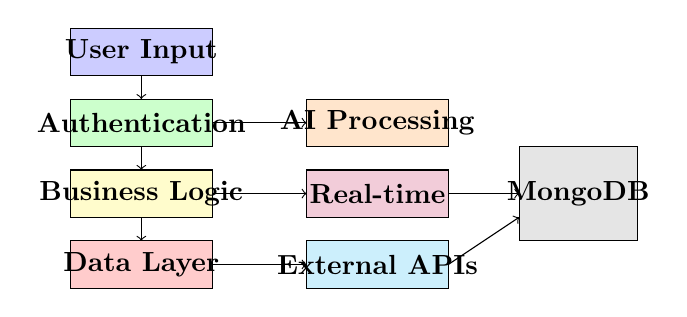
\begin{tikzpicture}[scale=0.6]
% Input Layer
\draw[fill=blue!20] (1,7) rectangle (4,8);
\node at (2.5,7.5) {\textbf{User Input}};

% Authentication Layer
\draw[fill=green!20] (1,5.5) rectangle (4,6.5);
\node at (2.5,6) {\textbf{Authentication}};

% Business Logic Layer
\draw[fill=yellow!20] (1,4) rectangle (4,5);
\node at (2.5,4.5) {\textbf{Business Logic}};

% AI Processing Layer
\draw[fill=orange!20] (6,5.5) rectangle (9,6.5);
\node at (7.5,6) {\textbf{AI Processing}};

% Real-time Layer
\draw[fill=purple!20] (6,4) rectangle (9,5);
\node at (7.5,4.5) {\textbf{Real-time}};

% Data Layer
\draw[fill=red!20] (1,2.5) rectangle (4,3.5);
\node at (2.5,3) {\textbf{Data Layer}};

% External APIs
\draw[fill=cyan!20] (6,2.5) rectangle (9,3.5);
\node at (7.5,3) {\textbf{External APIs}};

% Database
\draw[fill=gray!20] (10.5,3.5) rectangle (13,5.5);
\node at (11.75,4.5) {\textbf{MongoDB}};

% Arrows
\draw[->] (2.5,7) -- (2.5,6.5);
\draw[->] (2.5,5.5) -- (2.5,5);
\draw[->] (4,4.5) -- (6,4.5);
\draw[->] (4,6) -- (6,6);
\draw[->] (2.5,4) -- (2.5,3.5);
\draw[->] (9,4.5) -- (10.5,4.5);
\draw[->] (9,3) -- (10.5,4);
\draw[->] (4,3) -- (6,3);
\end{tikzpicture}
\end{center}
\end{frame}ngle (7,5.5);
\node at (5.5,5) {\textbf{AI Processing}};

% Real-time Layer
\draw[fill=purple!20] (4,3) rectangle (7,4);
\node at (5.5,3.5) {\textbf{Real-time Comm}};

% Data Layer
\draw[fill=red!20] (0,1.5) rectangle (3,2.5);
\node at (1.5,2) {\textbf{Data Layer}};

% External APIs
\draw[fill=cyan!20] (4,1.5) rectangle (7,2.5);
\node at (5.5,2) {\textbf{External APIs}};

% Database
\draw[fill=gray!20] (8,2.5) rectangle (11,4);
\node at (9.5,3.25) {\textbf{MongoDB}};

% Arrows
\draw[->] (1.5,6) -- (1.5,5.5);
\draw[->] (1.5,4.5) -- (1.5,4);
\draw[->] (3,3.5) -- (4,3.5);
\draw[->] (3,5) -- (4,5);
\draw[->] (1.5,3) -- (1.5,2.5);
\draw[->] (7,3.5) -- (8,3.5);
\draw[->] (7,2) -- (8,2.5);
\draw[->] (3,2) -- (4,2);
\end{tikzpicture}
\end{center}
\end{frame}

% Slide 12: Research Methodology - Approach & Algorithm
\begin{frame}{Research Methodology - Approach \& Algorithm}
\textbf{Development Approach:}
\begin{itemize}
\item \textbf{Agile Methodology:} Iterative development with continuous feedback
\item \textbf{Full-Stack Development:} Integrated frontend and backend development
\item \textbf{API-First Design:} RESTful APIs for modular architecture
\item \textbf{Component-Based Architecture:} Reusable React components
\end{itemize}

\vspace{0.5em}
\textbf{AI Integration Algorithm:}
\begin{itemize}
\item \textbf{Step 1:} User query preprocessing and context analysis
\item \textbf{Step 2:} Intent classification using NLP models
\item \textbf{Step 3:} OpenAI API integration for intelligent responses
\item \textbf{Step 4:} Real-time translation using Google Translate API
\item \textbf{Step 5:} Response optimization and delivery
\end{itemize}

\vspace{0.5em}
\textbf{Authentication Flow:}
\begin{itemize}
\item JWT-based stateless authentication with refresh tokens
\item Role-based access control (RBAC) implementation
\item Secure password hashing using bcrypt
\end{itemize}
\end{frame}

% Slide 13: Research Methodology - Tools & Software
\begin{frame}{Research Methodology - Tools \& Software}
\begin{columns}
\begin{column}{0.5\textwidth}
\textbf{Development Tools:}
\begin{itemize}
\item \textbf{IDE:} Visual Studio Code
\item \textbf{Version Control:} Git \& GitHub
\item \textbf{Package Manager:} npm
\item \textbf{API Testing:} Postman
\item \textbf{Database GUI:} MongoDB Compass
\end{itemize}

\textbf{Design Tools:}
\begin{itemize}
\item \textbf{UI/UX:} Figma
\item \textbf{Diagrams:} Draw.io
\item \textbf{Icons:} Lucide React
\end{itemize}
\end{column}
\begin{column}{0.5\textwidth}
\textbf{Deployment Tools:}
\begin{itemize}
\item \textbf{Containerization:} Docker
\item \textbf{Web Server:} Nginx
\item \textbf{Process Manager:} PM2
\item \textbf{Environment:} Node.js Runtime
\end{itemize}

\textbf{Testing Tools:}
\begin{itemize}
\item \textbf{Unit Testing:} Jest
\item \textbf{Integration Testing:} Supertest
\item \textbf{Frontend Testing:} React Testing Library
\end{itemize}

\textbf{Monitoring:}
\begin{itemize}
\item \textbf{Logging:} Winston
\item \textbf{Error Tracking:} Custom middleware
\end{itemize}
\end{column}
\end{columns}
\end{frame}

% Slide 14: Tech Stack
\begin{frame}{System Architecture - Tech Stack}
\begin{columns}
\begin{column}{0.5\textwidth}
\textbf{Frontend:}
\begin{itemize}
\item React.js
\item Tailwind CSS
\item Socket.io Client
\item React i18next
\end{itemize}

\textbf{Backend:}
\begin{itemize}
\item Node.js
\item Express.js
\item Socket.io
\item MongoDB Atlas
\end{itemize}
\end{column}
\begin{column}{0.5\textwidth}
\textbf{AI \& APIs:}
\begin{itemize}
\item OpenAI API
\item Google Cloud Translate
\item TensorFlow.js
\end{itemize}

\textbf{Deployment:}
\begin{itemize}
\item Docker
\item Nginx
\item JWT Authentication
\end{itemize}
\end{column}
\end{columns}
\end{frame}

% Slide 6: System Architecture Diagram
\begin{frame}{System Architecture Diagram}
\begin{center}
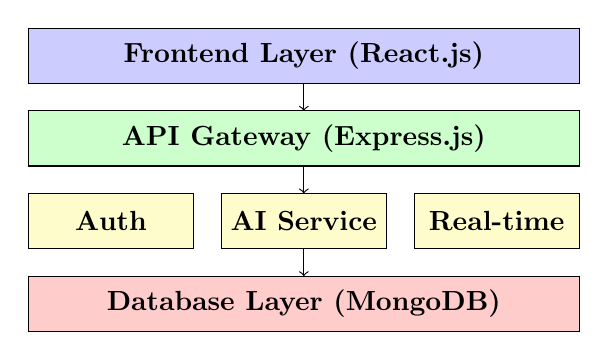
\begin{tikzpicture}[scale=0.7]
% Frontend Layer
\draw[fill=blue!20] (0,4) rectangle (10,5);
\node at (5,4.5) {\textbf{Frontend Layer (React.js)}};

% API Gateway
\draw[fill=green!20] (0,2.5) rectangle (10,3.5);
\node at (5,3) {\textbf{API Gateway (Express.js)}};

% Services Layer
\draw[fill=yellow!20] (0,1) rectangle (3,2);
\node at (1.5,1.5) {\textbf{Auth}};

\draw[fill=yellow!20] (3.5,1) rectangle (6.5,2);
\node at (5,1.5) {\textbf{AI Service}};

\draw[fill=yellow!20] (7,1) rectangle (10,2);
\node at (8.5,1.5) {\textbf{Real-time}};

% Database Layer
\draw[fill=red!20] (0,-0.5) rectangle (10,0.5);
\node at (5,0) {\textbf{Database Layer (MongoDB)}};

% Arrows
\draw[->] (5,4) -- (5,3.5);
\draw[->] (5,2.5) -- (5,2);
\draw[->] (5,1) -- (5,0.5);
\end{tikzpicture}
\end{center}
\end{frame}

% Slide 7: Admin Features
\begin{frame}{Key Features - Admin Dashboard}
\begin{itemize}
\item \textbf{Teacher Management}
  \begin{itemize}
  \item Add, edit, delete teachers
  \item Assign subjects and classes
  \end{itemize}
\item \textbf{Student Management}
  \begin{itemize}
  \item Complete student lifecycle management
  \item Enrollment and performance tracking
  \end{itemize}
\item \textbf{Analytics Dashboard}
  \begin{itemize}
  \item Real-time statistics and metrics
  \item Usage analytics and reports
  \end{itemize}
\item \textbf{System Logs \& Reports}
  \begin{itemize}
  \item Activity tracking and audit trails
  \end{itemize}
\end{itemize}
\end{frame}

% Slide 8: Teacher Features
\begin{frame}{Key Features - Teacher Portal}
\begin{itemize}
\item \textbf{Virtual Classroom}
  \begin{itemize}
  \item Live video sessions with WebRTC
  \item Screen sharing and interactive tools
  \end{itemize}
\item \textbf{Quiz Management}
  \begin{itemize}
  \item Create custom quizzes with auto-grading
  \item Performance analysis and feedback
  \end{itemize}
\item \textbf{Class Management}
  \begin{itemize}
  \item Student roster and attendance tracking
  \item Grade management and progress monitoring
  \end{itemize}
\item \textbf{Real-time Communication}
  \begin{itemize}
  \item Chat and collaboration tools
  \end{itemize}
\end{itemize}
\end{frame}

% Slide 9: Student Features
\begin{frame}{Key Features - Student Hub}
\begin{itemize}
\item \textbf{Virtual Classes}
  \begin{itemize}
  \item Join live sessions with real-time translation
  \item Interactive participation tools
  \end{itemize}
\item \textbf{AI Tutor}
  \begin{itemize}
  \item ChatGPT-powered 24/7 academic assistance
  \item Personalized learning support
  \end{itemize}
\item \textbf{Virtual Code Editor}
  \begin{itemize}
  \item Online coding environment
  \item Multiple programming language support
  \end{itemize}
\item \textbf{Materials \& Assessments}
  \begin{itemize}
  \item Access notes, quizzes, and proctored exams
  \end{itemize}
\end{itemize}
\end{frame}

% Slide 10: AI Integration
\begin{frame}{AI Integration}
\begin{center}
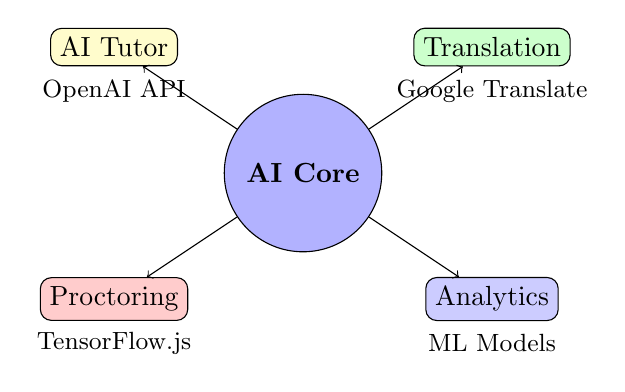
\begin{tikzpicture}[scale=0.8]
% Central AI node
\node[draw,circle,fill=blue!30,minimum size=2cm] (ai) at (0,0) {\textbf{AI Core}};

% Feature nodes
\node[draw,rounded corners,fill=yellow!20] (tutor) at (-3,2) {AI Tutor};
\node[draw,rounded corners,fill=green!20] (translate) at (3,2) {Translation};
\node[draw,rounded corners,fill=red!20] (proctor) at (-3,-2) {Proctoring};
\node[draw,rounded corners,fill=blue!20] (analytics) at (3,-2) {Analytics};

% Connections
\draw[->] (ai) -- (tutor);
\draw[->] (ai) -- (translate);
\draw[->] (ai) -- (proctor);
\draw[->] (ai) -- (analytics);

% Labels
\node at (-3,1.3) {\small OpenAI API};
\node at (3,1.3) {\small Google Translate};
\node at (-3,-2.7) {\small TensorFlow.js};
\node at (3,-2.7) {\small ML Models};
\end{tikzpicture}
\end{center}
\end{frame}

% Slide 11: Implementation - Database
\begin{frame}{Implementation - Database Schema}
\begin{columns}
\begin{column}{0.5\textwidth}
\textbf{User Model:}
\begin{itemize}
\item username, password
\item role (admin/teacher/student)
\item fullName, email
\item isActive, refreshToken
\end{itemize}

\textbf{Teacher Model:}
\begin{itemize}
\item userId (reference)
\item qualifications
\item subjects, assignedClasses
\end{itemize}
\end{column}
\begin{column}{0.5\textwidth}
\textbf{Student Model:}
\begin{itemize}
\item userId (reference)
\item enrollNo, standard
\item parentsContact, address
\end{itemize}

\textbf{Additional Models:}
\begin{itemize}
\item Quiz, Classroom
\item Authentication tokens
\item Activity logs
\end{itemize}
\end{column}
\end{columns}
\end{frame}

% Slide 12: Demo
\begin{frame}{Demo \& Testing}
\begin{center}
\textbf{Demo Credentials:}
\begin{tabular}{|c|c|c|}
\hline
\textbf{Role} & \textbf{Username} & \textbf{Password} \\
\hline
Admin & admin & admin123 \\
\hline
Teacher & teacher1 & teacher123 \\
\hline
Student & student1 & student123 \\
\hline
\end{tabular}
\end{center}

\vspace{1em}
\textbf{Access Points:}
\begin{itemize}
\item Frontend: \texttt{http://localhost:3000}
\item Backend API: \texttt{http://localhost:5000}
\item Login Page: \texttt{./login.html}
\end{itemize}
\end{frame}

% Slide 13: Deployment
\begin{frame}{Deployment}
\textbf{Docker Deployment:}
\begin{itemize}
\item Containerized application with Docker Compose
\item Nginx reverse proxy for production
\item Environment-based configuration
\end{itemize}

\textbf{Environment Setup:}
\begin{itemize}
\item MongoDB URI configuration
\item OpenAI API key integration
\item Google Translate API setup
\item JWT secret configuration
\end{itemize}

\textbf{Quick Start:}
\begin{itemize}
\item \texttt{docker-compose up -d}
\item Automated dependency installation
\item Production-ready deployment
\end{itemize}
\end{frame}

% Slide 14: Future Scope - Work Extensions
\begin{frame}{Future Scope - How the Work Can Be Extended}
\textbf{Platform Extensions:}
\begin{itemize}
\item \textbf{Mobile Application:} Native iOS/Android apps with offline capabilities
\item \textbf{Multi-Institutional Support:} Expand to support multiple educational institutions
\item \textbf{Advanced AI Models:} Integration with GPT-4, Claude, and custom-trained models
\item \textbf{Blockchain Integration:} Secure credential verification and certificate management
\end{itemize}

\textbf{Feature Enhancements:}
\begin{itemize}
\item \textbf{AR/VR Learning:} Immersive virtual classrooms and 3D educational content
\item \textbf{IoT Integration:} Smart classroom devices and environmental monitoring
\item \textbf{Advanced Analytics:} Predictive learning analytics and performance forecasting
\item \textbf{Gamification:} Learning badges, leaderboards, and achievement systems
\end{itemize}

\textbf{Technical Scaling:}
\begin{itemize}
\item \textbf{Microservices Architecture:} Decompose into independent, scalable services
\item \textbf{Multi-Cloud Deployment:} AWS, Azure, and Google Cloud integration
\end{itemize}
\end{frame}

% Slide 15: Future Scope - Further Improvements
\begin{frame}{Future Scope - Suggestions for Further Improvements}
\textbf{AI \& Machine Learning:}
\begin{itemize}
\item \textbf{Personalized Learning Paths:} AI-driven curriculum customization
\item \textbf{Emotion Recognition:} Detect student engagement and emotional states
\item \textbf{Advanced Proctoring:} Behavioral analysis and cheating detection
\item \textbf{Natural Language Processing:} Better understanding of student queries
\end{itemize}

\textbf{User Experience:}
\begin{itemize}
\item \textbf{Voice Interface:} Voice commands and audio-based interactions
\item \textbf{Accessibility Features:} Support for visually/hearing impaired users
\item \textbf{Offline Mode:} Content synchronization for low-connectivity areas
\item \textbf{Progressive Web App:} Enhanced mobile web experience
\end{itemize}

\textbf{Integration \& Interoperability:}
\begin{itemize}
\item \textbf{LTI Compliance:} Learning Tools Interoperability standards
\item \textbf{Third-party Integrations:} Zoom, Microsoft Teams, Google Workspace
\item \textbf{API Ecosystem:} Open APIs for third-party developers
\end{itemize}
\end{frame}

% Slide 16: Future Scope - Real-world Implications
\begin{frame}{Future Scope - Real-world Implications}
\textbf{Educational Impact:}
\begin{itemize}
\item \textbf{Digital Divide Reduction:} Bridging technology gaps in rural areas
\item \textbf{Personalized Education:} Adaptive learning for diverse student needs
\item \textbf{Teacher Empowerment:} AI-assisted teaching and administrative efficiency
\item \textbf{Global Accessibility:} Breaking geographical barriers to quality education
\end{itemize}

\textbf{Societal Benefits:}
\begin{itemize}
\item \textbf{Skill Development:} Preparing students for digital economy jobs
\item \textbf{Inclusive Learning:} Supporting students with special needs
\item \textbf{Cost Reduction:} Lower educational delivery costs for institutions
\item \textbf{Quality Standardization:} Consistent educational standards across regions
\end{itemize}

\textbf{Economic Implications:}
\begin{itemize}
\item \textbf{EdTech Market Growth:} Contributing to the \$350B+ global EdTech market
\item \textbf{Job Creation:} New opportunities in AI-education sector
\item \textbf{Institutional Efficiency:} Reduced operational costs for educational institutions
\item \textbf{Innovation Catalyst:} Inspiring further educational technology innovations
\end{itemize}
\end{frame}

% Slide 17: Conclusion
\begin{frame}{Conclusion}
\textbf{Key Achievements:}
\begin{itemize}
\item Comprehensive educational ecosystem with role-based access
\item AI-powered intelligent tutoring and assistance
\item Real-time communication and collaboration features
\item Scalable architecture with modern technology stack
\item Bilingual support for diverse user base
\item Responsive design for multiple devices
\end{itemize}

\vspace{1em}
\textbf{Impact:} Transforming traditional education through innovative technology solutions that enhance learning experiences for all stakeholders.

\vspace{1em}
\begin{center}
\textbf{Thank You!}\\
\textbf{Questions \& Discussion}
\end{center}
\end{frame}

\end{document}